\documentclass[letterpaper]{article}

\usepackage{natbib,alifeconf}  %% The order is important

% *****************
%  TODOs:
% *****************
% [ ] Writing: Abstract
% [ ] Writing: Results & discussion
% [ ] Writing: Conclusions
% [ ] Big 'ol citation pass: need to work appropriate citations into paper


% *****************
%  Requirements:
% *****************
%
% - All pages sized consistently at 8.5 x 11 inches (US letter size).
% - PDF length <= 8 pages for full papers, <=2 pages for extended
%    abstracts.
% - Abstract length <= 250 words.
% - No visible crop marks.
% - Images at no greater than 300 dpi, scaled at 100%.
% - Embedded open type fonts only.
% - All layers flattened.
% - No attachments.
% - All desired links active in the files.

% Note that the PDF file must not exceed 5 MB if it is to be indexed
% by Google Scholar. Additional information about Google Scholar
% can be found here:
% http://www.google.com/intl/en/scholar/inclusion.html.


% If your system does not generate letter format documents by default,
% you can use the following workflow:
% latex example
% bibtex example
% latex example ; latex example
% dvips -o example.ps -t letterSize example.dvi
% ps2pdf example.ps example.pdf


% For pdflatex users:
% The alifeconf style file loads the "graphicx" package, and
% this may lead some users of pdflatex to experience problems.
% These can be fixed by editing the alifeconf.sty file to specify:
% \usepackage[pdftex]{graphicx}
%   instead of
% \usepackage{graphicx}.
% The PDF output generated by pdflatex should match the required
% specifications and obviously the dvips and ps2pdf steps become
% unnecessary.


% Note:  Some laser printers have a serious problem printing TeX
% output. The use of ps type I fonts should avoid this problem.


\title{Understanding fine temporal scale evolutionary dynamics with lineage metrics}
\author{Emily Dolson$^{1,2,3}$, Alexander Lalejini$^{1,2, 3}$, Steven Jorgensen$^{1,2}$ \and Charles Ofria$^{1,2, 3}$ \\
\mbox{}\\
$^1$BEACON Center for the Study of Evolution in Action, Michigan State University, East Lansing, MI, 48824 \\
$^2$Department of Computer Science and Engineering, Michigan State University, East Lansing, MI, 48824 \\
$^3$Ecology, Evolutionary Biology, and Behavior Program, Michigan State University, East Lansing, MI, 48824 \\
dolsonem@msu.edu} % email of corresponding author

% For several authors from the same institution use the same number to
% refer to one address.
%
% If the names do not fit well on one line use
%         Author 1, Author 2 ... \\ {\Large\bf Author n} ...\\ ...
%
% If the title and author information do not fit in the area
% allocated, place \setlength\titlebox{<new height>} after the
% \documentclass line where <new height> is 2.25in



\begin{document}
\maketitle

\begin{abstract}

\end{abstract}

\section{Introduction}

Evolution is an emergent effect of events (\textit{e.g.} replication, variation, and competition) that occur on a much finer-grained temporal scale. While evolution's emergent nature is a large part of why it is so fascinating, it also presents challenges to studying the short-term mechanisms that govern long-term results. In computational evolutionary systems, we theoretically have adequate data to untangle these mechanisms. In practice, though, gathering appropriate data to do so can be challenging. Moreover, because of the vast difference between the scales that evolutionary causes and effects can occur on, the quantity of such data can be overwhelming. Both of these problems can be mitigated with a standardized set of diagnostic summary metrics that paint a picture of shorter-term evolutionary dynamics within a population. Here, we suggest a suite of metrics that operate on lineages and phylogenies. We then use experimental results to provide an intuition for what they can tell us about evolution.

A lineage describes a continuous line of descent, linking ancestors and their descendants. A complete lineage can provide a post-hoc, step-by-step guide to the evolution of an extant organism where each step involves replication and inherited variation. Indeed, lineage analyses are a powerful tool for disentangling evolutionary dynamics in both natural and digital systems; digital systems, however, allow for fine-grained lineage tracking at resolutions that are impossible in modern wet lab experiments, allowing us to replay the tape of life in exacting detail and to tease apart the evolutionary recipe for whatever complex feature or phenomenon we happen to be interested in~\citep{mcphee_using_2016}. 
In a more famous example, Lenski \textit{et al.}, used the lineage of an evolved digital organism in Avida to tease apart, step-by-step how a complex feature (the capacity to perform the equals logical operation) emerged~\citep{lenski_evolutionary_2003}. 

Yet, tracking the full details of a single lineage, much less a population of lineages, can be computationally expensive and will inevitably generate an unwieldy amount of data that can be challenging to visualize and interpret~\citep{mcphee_visualizing_2016}.
Summary statistics can help alleviate these issues by enabling the user to focus on aggregate trends across a population rather than needing to examine each individual's lineage. The question is how to effectively summarize what is essentially a path through fitness space. A useful abstraction is to treat the path as a sequence of states. Here, we will use phenotypes and genotypes as the states in the sequence, but we could just as easily use some other descriptor of the lineage's position in the fitness landscape at a given point in time.
With this abstraction in hand, a few metrics are easily formalized: the number of unique states, the number of transitions between states, and the amount of time spent in each state. 
Additionally, we may care about how the transitions between states happened. What mutations lead to them? Were those mutations beneficial, deleterious, or neutral at the time? Here, we choose a subset of these metrics that we expect will be particularly useful to explore further.

Whereas a lineage represents the evolutionary history of a single individual, a phylogeny represents the evolutionary history of an entire population. Measurements that summarize phylogenies can provide useful insight into population-level evolutionary dynamics, such as diversification and co-existence among different clades. A variety of useful phylogeny measurements have already been developed by biologists~\citep{tucker_guide_2017}. These measurements tend to treat the phylogeny as a graph and make calculations about its topology. Tucker \textit{et al.} group them into three broad categories: assessments of the quantity of evolutionary history represented by a population, assessments of the amount of divergence within that evolutionary history, and assessments of the topological regularity of the phylogenetic tree. Such measurements can help quantify the behavior of the population as a whole, providing insight into interactions between its members. Thus, they are useful indicators of the presence of various types of eco-evolutionary dynamics.
%@AML: I think the next bit (just moved it) might belong in the metrics section. Instead, we might want a little more elaboration on each of the categories of metrics.
%@ELD: Is that too handwavy?
%@AML: Nah! Handwaving is just what we needed! 

Here, we present three types of lineage measurements: lineage length, mutation accumulation, and phenotypic volatility. Additionally, we suggest the adoption of four phylogeny measurements from biology: most-recent common ancestor depth, phylogenetic richness, phylogenetic divergence, and phylogenetic regularity. For each metric, we discuss its application and our intuitions for what it can tell us about evolution. We evaluate our intuitions on a set of two-dimensional, real-valued optimization problems under a range of mutation rates and selection strengths. For this work, we restrict our attention to asexually reproducing populations; however, we make suggestions as to how these metrics can be extended to sexual populations. 

%@AML:  It might be nice to wrap this section up with a little bit of a 'call to action'/'why should you care about this as a community'
In addition to demonstrating a range of metrics that are immediately applicable and useful to digital evolution research, we hope this work begins a conversation within the computational evolution community about how we quantify, interpret, and compare observed evolutionary histories. There has been extensive efforts to improve our ability to visualize both lineages and phylogenies [CITATIONS], which are incredibly valuable for building intuitions and qualitatively understanding the dynamics embedded in a population's evolutionary history. However, we are unaware of efforts to formalize a suite of quantitative lineage- and phylogeny-related metrics for computation evolution. Indeed, .... % people have done stuff with lineages
% - often a component of a larger experiment-specific analysis or limited to qualitative descriptions/visualizations
% - well-defined metrics not only provide valuable tools for teasing apart evolutionary dynamics, they also facilitate allow us to move away from exclusively qualitative descriptions/understandings of results ==> better quantitative understanding/statistics ==> better hypothesis testing
% - facilitate comparisons among systems. 
% - Something about activity metrics?

\section{Metrics}

Code for all of our metrics is open source and available in the Empirical library (https://github.com/devosoft/Empirical). Empirical is a C++ library built to facilitate writing efficient and easily sharable scientific software. To facilitate including useful features without excessive overhead, Empirical is header-only, meaning these metrics can be imported into an existing project with minimal effort.
% [QUESTION] @AML: Is it actually true that someone could include these metrics with minimal effort? How much of Empirical would it impose on the user? Just the systematics manager? 

\subsection{Lineage Metrics}
% Outlining some points to (maybe) make here; probably too bogged down in details; not even sure we want to talk about lineages as graphs:
% - Apply metrics in context of asexual populations
% - Establish a framework from which to think about metrics (not novel, but rarely formalized)
% 	 - We treat lineages as sequences of states where each state represents an individual and transitions between states represent parent-offspring relationships.
%      - More formally, lineages are directed acyclic graphs where internal nodes have in-degree = 1 (parent), out-degree = 1 (offspring). Original ancestor (in digital evolution, often seed of population) w/out-degree = 1. Extant individual w/in-degree = 1.
%      - Transitions specify relevant variation introduced into offspring (e.g. mutations)
%      - States specify relevant genotype and phenotype information (e.g. genome, location in space, behavior, etc) -- anything we might want to measure over a lineage
%      - Becomes more complicated with sexual populations, but we'll stick with asexual assumption for this. 
%  - Already, framework affords certain questions:
%     - How many individuals are along the lineage? 
%     - Total # and magnitude of mutations along lineage?
%     - Distribution of mutation types (ins vs. sub/beneficial vs. deleterious)?
%  - Further abstractions:
%      - Sequence of genotypes along lineage (where each genotype may represent multiple individuals)
%      - Sequence of phenotypes along lineage (where each phenotype may represent multiple individuals)
%      - Still further abstraction: sequence of a particular aspect of genotype (e.g. genetic marker)/phenotype (e.g. location) along lineage
%  - We discuss three classes of lineage metrics within this framework: lineage length, mutation accumulation, and phenotypic volatility. 
%  - For each, we discuss our intuition for what they can tell us (alone and in combination) about evolution. 
Each of the three lineage metrics we discuss --- lineage length, mutation accumulation, and phenotypic volatility --- reduces a lineage to a linear sequence of states where each state represents an individual or a continuous sequence of individuals that share some common genotypic or phenotypic characteristic of interest. While we limit our focus to three lineage metrics, this abstraction places lineages in a form suitable for a wide range of measurements, including the direct application of many data mining techniques designed to operate over sequences such as sequential pattern mining, trend analysis, \textit{et cetera} \citep{han2011data}. 

Only lineages consisting of asexually reproducing ancestors where genetic material is exclusively vertically transmitted can be directly abstracted as a \textit{linear sequence} of states. 
Sexual reproduction (and any form of horizontal gene transfer) complicates matters significantly as such lineages are more appropriately represented by trees rooted at the extant organism, branching for each contributor of genetic material. 
For each metric we present here, we limit our discussion to asexual populations; however, we suggest two approaches for generalizing these lineage metrics to sexual populations: apply a lossy compression to reduce sexual lineages into linear sequences or extend our application of the metrics to operate over non-linear (tree) structured lineages. 
Sexual lineages can be compressed into linear sequences of states by modeling sexual reproduction events as asexual reproduction events, designating one parent to be a part of the lineage and considering the genetic contributions of other parents as sources of genetic variation (mutations). The primary downside to this approach is its lossy-ness (i.e. the fact that it discards potentially important parentage information). 
Alternatively, we can extend our metrics to operate over the more complex state sequences that constitute the lineages of sexually reproducing organisms. One such approach would be to consider all possible ancestor paths for an extant individual, calculating a given metric for each of them and then averaging the resulting values together. Assessing the efficacy of these and potentially other approaches would be a useful line of research to pursue in the future.

\subsubsection{Lineage Length}
% Define/explanation
% 	- Within context of framework, lineage length is simply measure of number of states in the graph/sequence.
%   - What this means will depend on what states represent?
%       - number of individuals along lineage 
%             - More interesting in experiments where generations are not dictated by system, but rather by life history strategies of organisms
%             - Give you a diagnostic for replication rate (r vs. k strategy)
%      - number of genotypes along lineage
%            - length = 1: no mutations
%            - length = number of individuals: mutation in every replication
%            - Intuitively, should be higher at high mutation rates, lower at low mutation rates. 
%      - number of phenotypes along lineage
%            - low: evidence for static environment
%            - high: might be indicative of a changing environment or ecological interactions
%            - if number of genotypes is high, but number of phenotypes low, probably in a neutral fitness landscape
%      - various subsets of genotype/phenotype
%           - location in space (environment type): useful for looking at lineage through heterogeneous landscape
%           - change in particular phenotypic trait
%           - change in genetic markers
%           - Distributions of above two lengths can tell you useful things about drift, selection, etc.

Lineage length describes the number of ancestral states traversed by a lineage. If a state represents a single individual along a lineage, lineage length is a measure of the number of generations on a lineage. This form of the lineage length metric is most useful in systems where generational turnover is not algorithmically determined but instead determined by the life history strategies of organisms. In these systems, lineage length can provide a proxy for replication rate where, for lineages that span equal lengths of time, longer lineages imply faster replication rates and shorter lineages imply slower replication rates. 
%@ELD: I've always heard these called r- and k- selected rather than replicator, but I'm totally willing to believe these terms are used too.
%@AML: Yup. I have no idea if I've ever heard them referred to as 'r-replicator vs. k-replicator'. I'm going to get rid of the two parentheticals for now.

Lineage length becomes an increasingly flexible and informative metric if we begin to consider more abstract definitions of an ancestral state along a lineage. 
We might measure lineage length where an ancestral state represents a temporally continuous sequence of individuals that share a phenotypic or genotypic characteristic of interest. In these cases, lineage length only increases if the characteristic of interest changes from parent to offspring. For example, in an environment where organisms must perform a set of tasks to be successful, we might define ancestral state to be the set of tasks performed by an individual (\textit{e.g.} the set of logic operations performed by a digital organism in the default logic 9 Avida environment). In this scenario, lineage length would only increase when the set of tasks performed by an ancestor changes, compressing sequential ancestors that perform the identical sets of tasks into a single ancestral state. 
% This could be made very clear with a good example here. 
%@ELD Maybe I'm just getting tired, but I didn't quite follow that last sentence
%@AML: It was definitely hard to follow. Hopefully it's better now? 
%  -- Still could use a sentence about what the measure might tell us in the given example. 

\subsubsection{Mutation Accumulation}
Mutation Accumulation defines a set of measurements that track mutational changes across a lineage. These changes can be measured in a variety of ways, such as the magnitude of the change (for real-valued genomes), or the total count of changes (for discrete-valued genomes). The type of a mutation can also be tracked, and can provide insight into the distribution of mutation types for a given lineage. Measures of mutation accumulation along the lineages of successful extant individuals can help to tease apart the relative importance of different types of mutational events when compared to what is expected by chance. 

In conjunction with collected fitness information, the class of a mutation (\textit{e.g.} beneficial, deleterious, or neutral) can also be tracked. Different evolutionary conditions are expected to cause different distributions of mutations along a lineage~\citep{barrick2013genome}; deviations revealed by measures of mutation accumulation can act as a barometer for unexpected evolutionary dynamics.   
The number and magnitude of deleterious mutations along a lineage can both tell us something about the ruggedness of the fitness landscape as well as how well a lineage was able to cross fitness valleys. 
Similarly, an elevated measure of neutral mutations relative to beneficial or deleterious mutations can tell us that the fitness landscape has a large neutral area that the lineage is spending most of its time drifting around. 



% Mutation accumulation over a lineage 
%  - Measured in a variety of ways
%   - For real-valued genomes, we can track magnitudes of changes
%   - For discrete-valued genomes, we can track counts of changes
%      - Track by type to get distribution of mutation types
%   - In conjunction with fitness information, can track classes of mutation: beneficial, deleterious, neutral
%      - Again, can extract a distribution; different environments/experiments, you might expect different distributions
%      - Importance of deleterious steps; valley crossing, etc

\subsubsection{Phenotypic Volatility}

Phenotypic volatility addresses the rate at which the lineage changes phenotype (although the same concept can be applied to other types of state). In systems with discrete/categorical phenotypes, this can be measured by summing the number of times the phenotype changes. A related but subtly different measurement in such systems is the number of unique phenotypes on a lineage. In most cases, these values will be very similar. A discrepancy between them, however, would be a clear signal of interesting dynamics. Specifically, it would suggest that the lineage was in a portion of the landscape where it could rapidly switch among different phenotypes. Such behavior could be indicative of some form of evolutionary bet-hedging.

In systems with continuous-valued phenotypes, a subtly different approach is needed to measure phenotypic volatility, because there are no discrete state transitions. Instead, we can measure the overall variance in phenotype along a lineage. In some cases, it may be desirable to smooth out the noise inherent in a real-valued phenotype. We can do so by instead taking the variance of the rolling mean of fitness, to more closely approximate the idea of measuring phase transitions.
% TODO

% Define/describe
% .... 
% Useful things that this metric could identify:
% - Mutational bet hedging (high volatility)
% - Plasticity (high volatility)
% - Neutral landscapes (expect low volatility)

% Here, we... 

\subsubsection{Summary statistics}

Each of these metrics can be calculated for each member of the population at each time step. Doing so, however, would produce an amount of data so large that it would be difficult to make sense of. Instead, we need to come up with ways to generate useful summaries. There are two main approaches to doing so: 1) choose a small number of representative lineages from a given time point, 2) collect summary statistics about the distribution of metric values across the population.

A single representative lineage can be chosen by selecting the lineage of the dominant organism (either the most fit or the more numerous; here we use the most fit). In populations with a diversity of coexisting strategies this approach can be uninformative as the dominant lineage is not necessarily representative of all successful lineages. An alternative in these scenarios is to filter out lineages that do not have offspring some predetermined number of generations later as such lineages were likely not representative of an important subset of the population. Still, any approach based on measuring only a subset of lineages can be challenging to interpret when the current dominant lineage (or lineages) is replaced with a different one; such changes can introduce a discontinuity if the value is being measured over time. If graceful responses to changes in which lineage is dominant are required, it can be advantageous to instead measure summary statistics (e.g. mean, variance, and range) across the entire population. 

In scenarios where selective sweeps happen rapidly, the dominant lineage will likely be very similar to the average lineage in the population, as most of the population will be closely related. When the population contains more phylogenetic diversity, however, it is possible for the dominant lineage to differ from the mean. The nature of such differences is likely informative about the evolutionary dynamics occurring in the population. Since we have yet to observe an instance of this phenomenon, we do not explore it further in this paper. Nevertheless, it presents an argument for measuring the dominant lineage in addition to gathering summary statistics across the population.


\subsection{Phylogeny metrics}

These metrics operate on entire phylogenies rather than single lineages within a population. Thus, in most cases, summarizing them across the population is not an issue as it is with lineage metrics. Because they factor in the entire population, phylogeny metrics can be more computationally expensive to calculate than metrics about a single lineage. On the other hand, because most lineages in the population share a substantial amount of history, phylogeny metrics can often be calculated more rapidly than lineage metrics can be calculated across an entire population. Note that phylogenies can be constructed with regard to any taxonomic level of organization, be it individual, genotype, phenotype, etc. Thus, when we refer to items in a phylogeny, we will use the term \textit{taxa}.

A standard technique for saving memory and time when working with lineages in computational systems is to "prune" them, removing any taxa that are not either currently alive or the ancestor of taxa that are alive. Since all of the phylogeny metrics we discuss here are borrowed from natural systems (where we do not have information about taxa without offspring), they all are designed to work on pruned phylogenies. Thus, for the remainder of this paper, we will assume we are only working with pruned phylogenies.

In populations without ecological forces promoting coexistence, phylogenies should coalesce periodically, resulting in pruned lineages that mostly consist of a single path. When there is strong selection, this coalescence should happen even more rapidly. Thus, phylogenies with topologies that deviate from that expectation are an indication of ecological interactions within the population. The metrics discussed here can provide insight into the nature of those interactions and their long-term evolutionary effects. As a result, they are often referred to as phylogenetic diversity metrics~\citep{tucker_guide_2017}.

An important distinction between phylogenies in natural vs computational systems to be aware of is that in natural systems phylogenies are generally inferred from extant taxa, whereas in computational systems they are directly measured. The inferred phylogenies used in natural systems do not contain internal nodes unless those nodes are branch points. They also do not contain history prior to the most recent common ancestor (MRCA) of all organisms in the extant population. For consistency, we will exclude pre-MRCA taxa from our analyses. However, we will not remove non-branching internal nodes, as these only serve to make our phylogenies more informative.

Here we provide a high-level summary of phylogeny metrics that we expect will be particularly useful. For more metrics and more detail on all of these metrics, see~\citep{winter_phylogenetic_2013, tucker_guide_2017}. 

\subsubsection{Depth of Most-Recent Common Ancestor}

The depth of the MRCA (i.e. how many steps from the beginning of time did it occur?) is a useful metric because of the relatively high ratio of informativeness to ease of calculation. A more recent MRCA implies more frequent selective sweeps and less long-term stable coexistence between clades. The depth of the MRCA is so easily calculated because most any implementation of phylogeny pruning requires keeping track of it already. Measuring the frequency with which the MRCA changes (i.e. the number of coalescence events) can also by informative, as some conditions can inflate the length of the lineage relative to other conditions, without actually increasing the frequency of selective sweeps. This scenario is particularly likely when the population size is changing over time. A downside to the depth of MRCA as a metric is that any population that does have a stable ecology will likely never see a change in the MRCA after the very beginning of evolution.

\subsubsection{Phylogenetic Richness}

Measurements of phylogenetic richness quantify the total amount of evolutionary history that is contained in a set of taxa. The most traditional metric of phylogenetic richness is the one simply titled "Phylogenetic Diversity", which is calculated as the number of the nodes in the minimum spanning tree from the MRCA to all extant taxa~\citep{faith_conservation_1992}. Another approach is to calculate the pairwise distances between all taxa and sum them~\citep{tucker_guide_2017}. A third approach is to calculate evolutionary distinctiveness, a measurement of a taxon's evolutionary uniqueness~\citep{isaac_mammals_2007}, and sum it across all extant taxa~\citep{tucker_guide_2017}.

\subsubsection{Phylogenetic Divergence}

Measurements of phylogenetic divergence quantify how distinct the taxa in the population are from each other, and are often the means of values that can be calculated for individual taxa. For instance, one option is to calculate the mean of the pairwise distances between all taxa in the population~\citep{webb_exploring_2000}. Similarly, phylogenetic divergence can also be calculated by calculating the evolutionary distinctiveness of each taxon in the population (as alluded to in the previous section) and taking the average of these values.

\subsubsection{Phylogenetic Regularity}

Measurements of phylogenetic regularity quantify how balanced the branches of the phylogeny are, and are often the variances of values that can be calculated for individual taxa. Just as the mean of the pairwise distances between all taxa in the population is a measurement of phylogenetic divergence, taking their variance is a measurement of phylogenetic regularity. The same is true of the variance of evolutionary distinctiveness across the population.

\section{Test Problems}
To understand the metrics defined above, the test problems used need to be well understood and studied. The benchmark functions from the GECCO Competition on Niching Methods meet both of these requirements and allow us to visualize the actual fitness landscape, due to the low dimensionality of the problems ~\citep{li_benchmark_2013}. For each problem, the X and Y coordinates offered by a given organism are translated by the function into a fitness value. We chose a diverse subset of these functions (Himmelblau, Shubert, Composition Function 2, and Six-Humped Camel Back) as our test problems in order to gain a broad understanding of our metrics. We used the implementations of these problems at https://github.com/mikeagn/CEC2013/ (C++ for fitness calculations during evolution, Python for post-hoc analysis). Figure \ref{TODO} shows the fitness landscapes defined by each of our four chosen test problems. 

% @AML: It would be neat to have a tournament size = population size treatment (pure hill climbing)
For each test problem, we evolved populations of 1000 digital organisms under a range of mutation rates and selection strengths for 5000 generations. Each digital organism's genome consisted of two floating point numbers that defined its position in the fitness landscape. To determine which organisms reproduced each generation, we used tournament selection. We evolved populations under five different tournament sizes: one, two, four, eight, and sixteen.  Tournament size represents strength of selection where higher tournament sizes correspond to a higher strength of selection and lower tournament sizes correspond to a lower strength of selection. A tournament size of one is equivalent to no selection pressure (\textit{i.e.} every organism in the population has an equal chance of being selected to reproduce). Organisms selected to reproduce did so asexually. Each value in an offspring's genome was mutated by adding noise given by a normal distribution with a mean of 0; the `mutation rate' of a treatment defined the standard deviation used to defined this normal distribution and was given as a proportion of the test problem's domain.  For each problem and tournament size, we evolved populations at eight mutation rates: \textbf{TODO}. 
% @AML: Don't love how I've phrased mutation rate sentences. 

% @AML: if room, it might be helpful to have a cartoon figure that gives all of our treatments
%		-- I'm imagining a table where we have axes/arrows that show 'increasing selection' vs. 'increasing mutation rate'

\section{Implementation}

\section{Data Analysis}
\subsection{3D visualizations}
% Trim dramatically
%Evolutionary biologists often accuse each other of making up "just-so" stories - post-hoc explanations for how an observed trait or pattern could have evolved. The problem with these stories is that, in biology, there is often no way to verify that they reflect what happened in biology. Due to evolution's stochastic nature, it is easy to come up with possible ways that something could have happened once, regardless of how repeatable they are. Theoretically, we should easily be able to avoid this problem in computational evolution by carefully checking the underlying assumptions behind our hypothesized explanation.  All too often, however, we fail to drill down to the true underlying mechanism behind an observed effect.

%The metrics we propose here can help provide a check on this behavior, by making information about underlying evolutionary dynamics more readily accessible. They can only have that effect, however, if we completely understand what they are telling us about the way populations under different conditions are traversing different fitness landscapes. In order for these metrics to be useful for diagnosing the behavior of an evolving population, we need to establish ground truth for what underlying evolutionary dynamics are implied by different values of the metrics. For the purposes of building this intuition on a solid foundation, we wanted to be able to visualize the full evolutionary history of each population as it traversed the fitness landscape.

%To this end, we chose problems for which we could perfectly visualize the fitness landscape, and kept track of the complete evolutionary history of all members of the population. With these data, we were able to overlay successful lineages on top of the fitness landscape. Visualizing all lineages in each experimental condition in this way gave us an efficient check on our understanding of the underlying evolutionary dynamics in that condition. 
In order to make these metrics useful in the long run, it is critical that we have an accurate understanding of how various measurements correspond to the actual behavior of lineages. The most direct way to confirm our expectations is to visualize the path that each lineage takes across the fitness landscape, mapping the x, y, and z (fitness) coordinates of each ancestor of each member of the population. Creating such a visualization entails incorporating a large quantity of information into a limited space. When projected onto two dimensions, lineages can obscure parts of the fitness landscape (and each other). To mitigate this problem, we built a thee-dimesnional visualization using the A-Frame Framework [cite].

A-Frame supports building three dimensional scenes and rendering them to a variety of platforms. In the simplest case, the visualization is rendered in WebGL, allowing it to be viewed in a standard web browser. Mouse interactions such as rotation make it possible to view the visualization from all angles, and WebGL's use of the graphics card allows it to render data-rich visualizations. A-Frame also supports rendering the page with WebVR, allowing it to be viewed using various virtual reality headsets. These platforms allow the user to explore the data in a truly three-dimensional environment. Different headsets support different amounts of interaction. For the data interpretation in this paper, we used an Oculus Rift to provide us with fine-grained control of which part of the visualization we were looking at.

\subsection{Metric analysis}

We analyzed trends in our metrics using the R Statistical Computing Language~\citep{r_core_team_r:_2017}. Specifically, we used the ggplot2 library for all graphs included in this paper~\citep{wickham_ggplot2:_2009}. All analysis scripts are available at https://github.com/stevenjson/ALife2018-Lineage.

\section{Results and Discussion}
% Changing mutation: here's what happens when we change mutation on each problem
\begin{figure*}
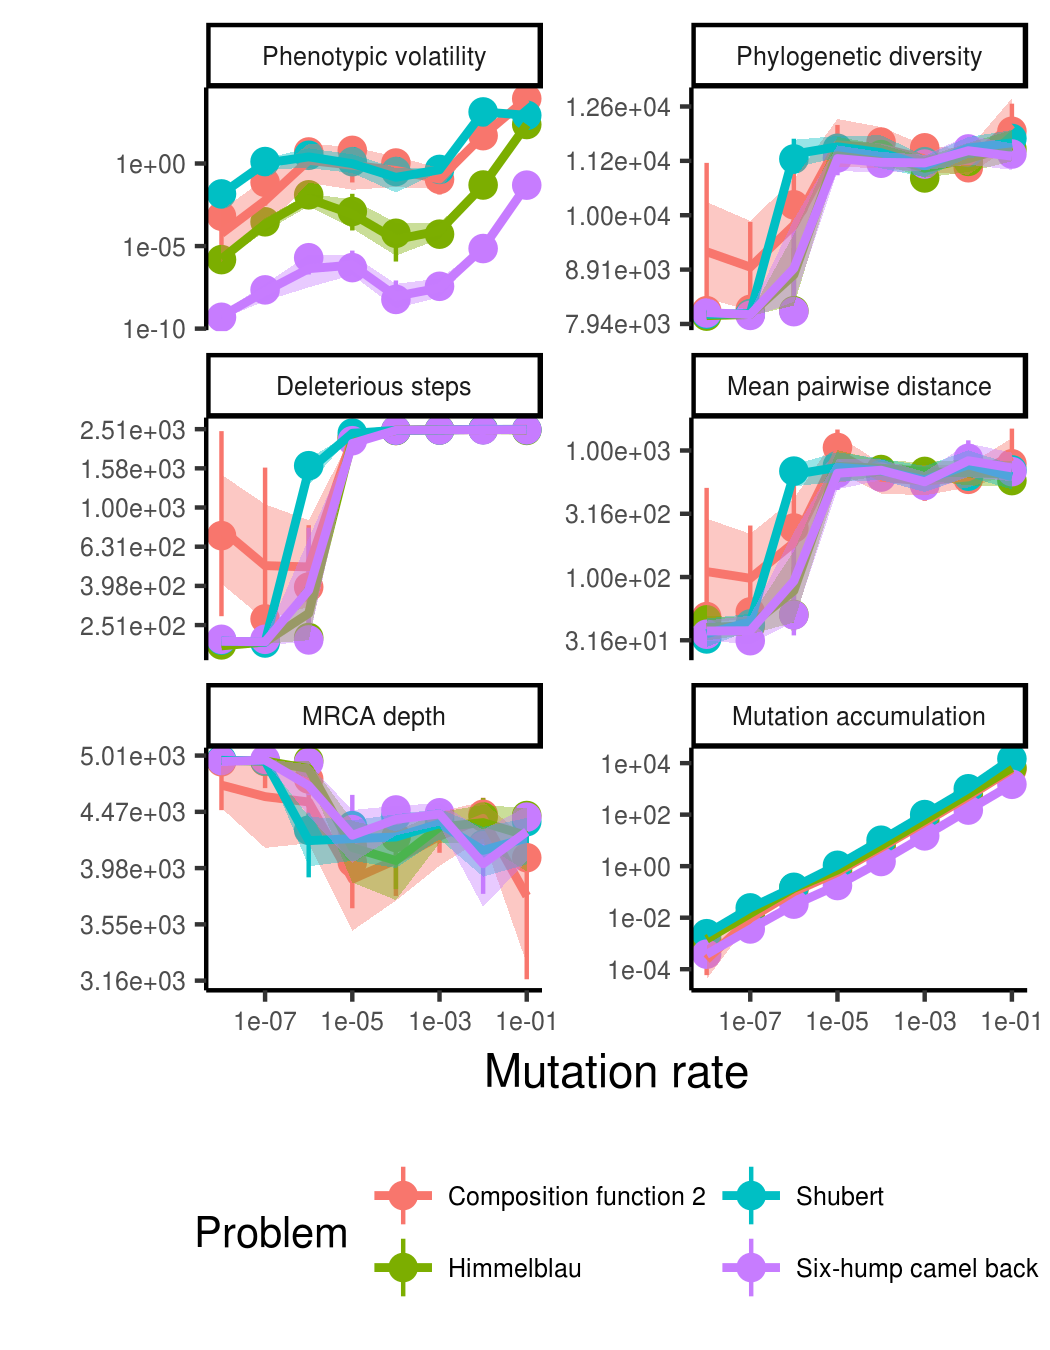
\includegraphics[width=7in]{figs/all_mutation_rate.png}
\caption{Values of example metrics across different mutation rates for each of the four problems. Circles are medians and vertical lines show inter-quartile range.}
\end{figure*}

% \begin{figure}
% 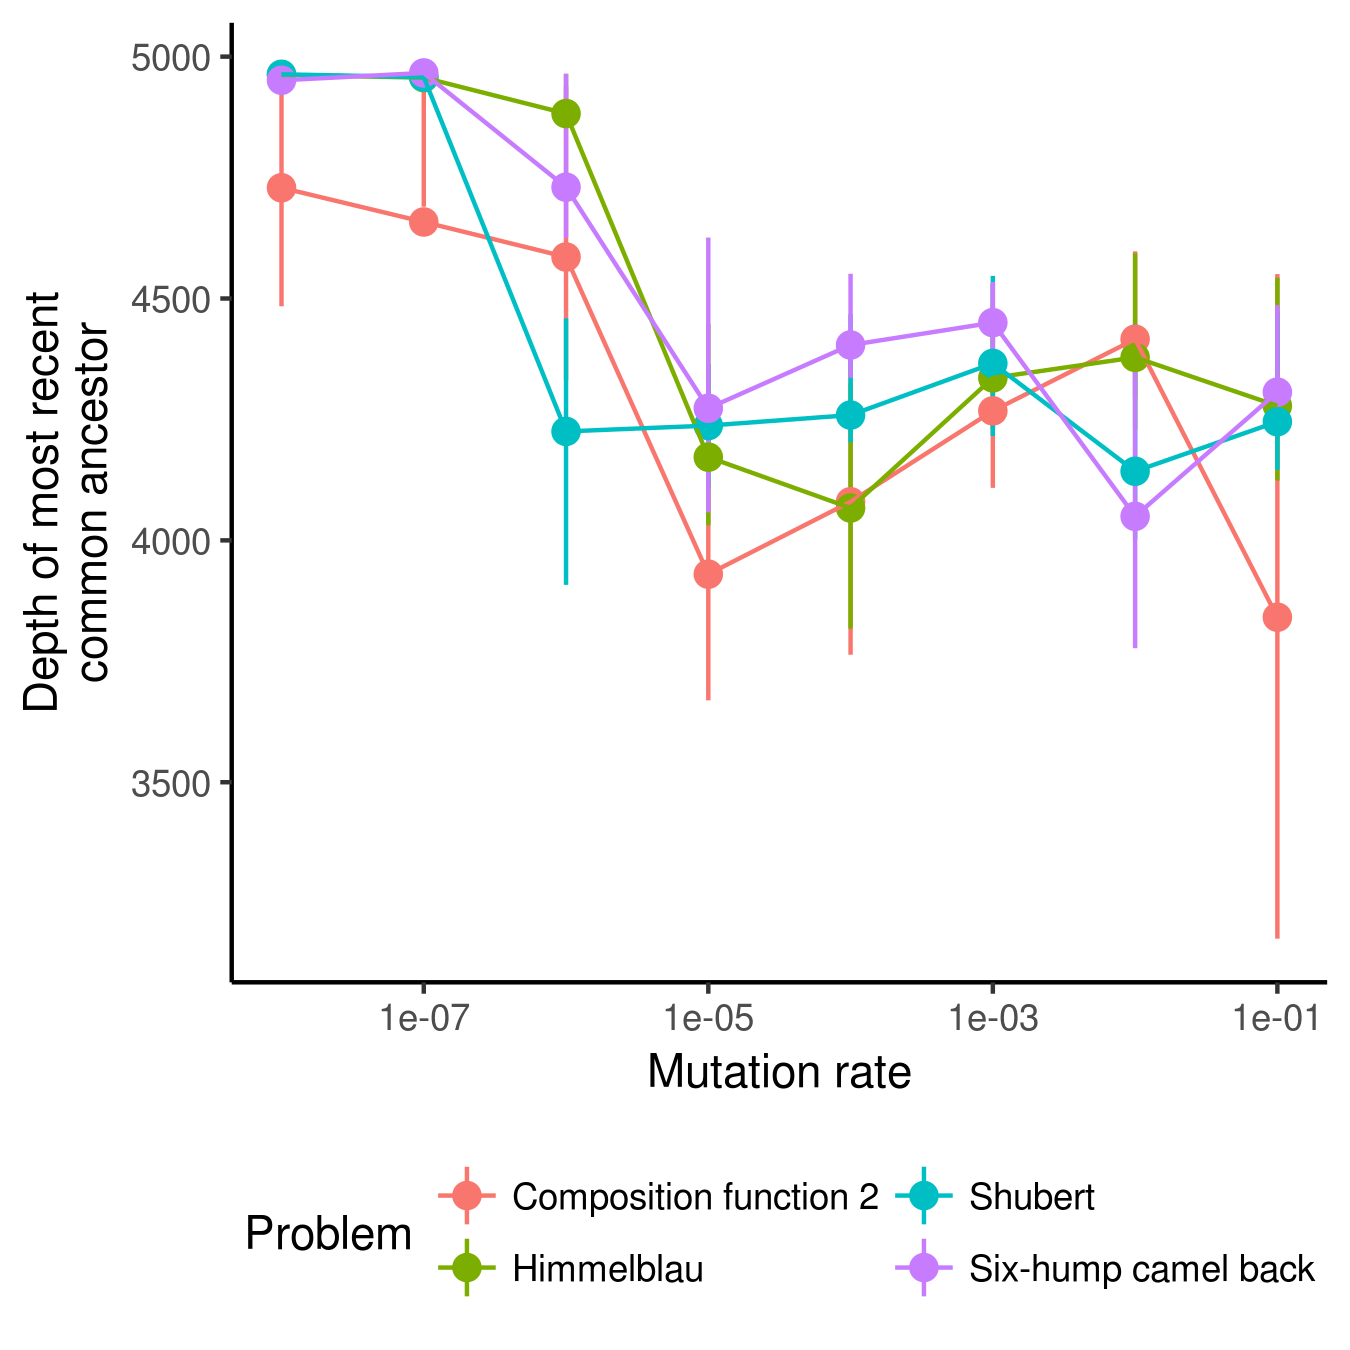
\includegraphics[width=3.5in]{figs/mrca_depth_mutation.png}
% \end{figure}

% \begin{figure}
% 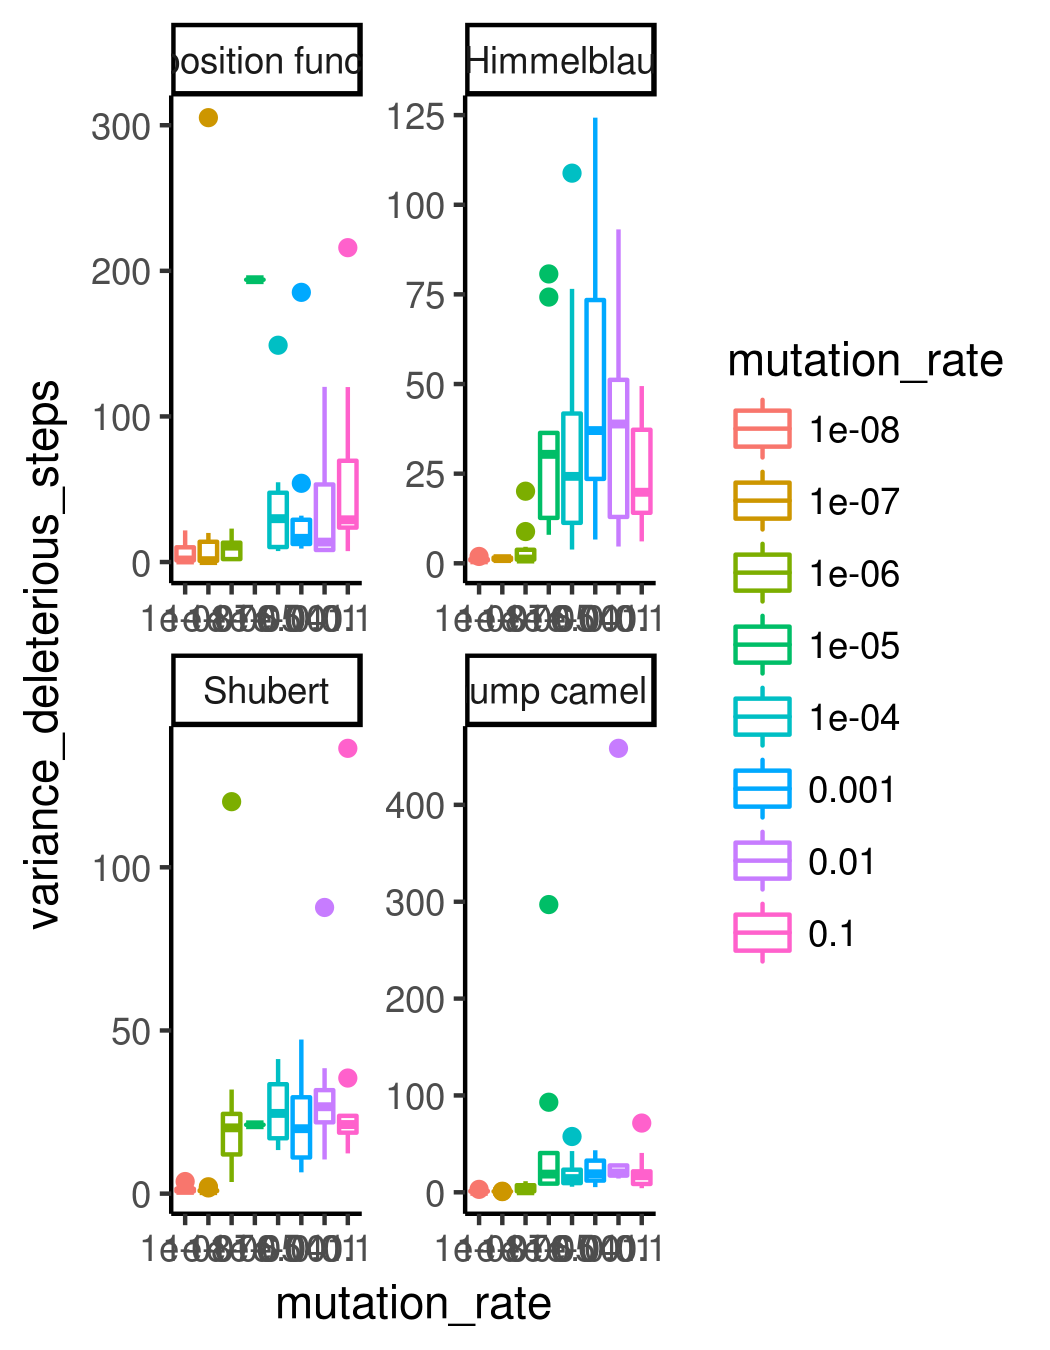
\includegraphics[width=3.5in]{figs/variance_deleterious_mutation_rate.png}
% \end{figure}

% - Metric 1
% Problem 1
% Problem 2
% Problem 3
% Problem 4
% - Metric 2
% ... 

\begin{figure*}
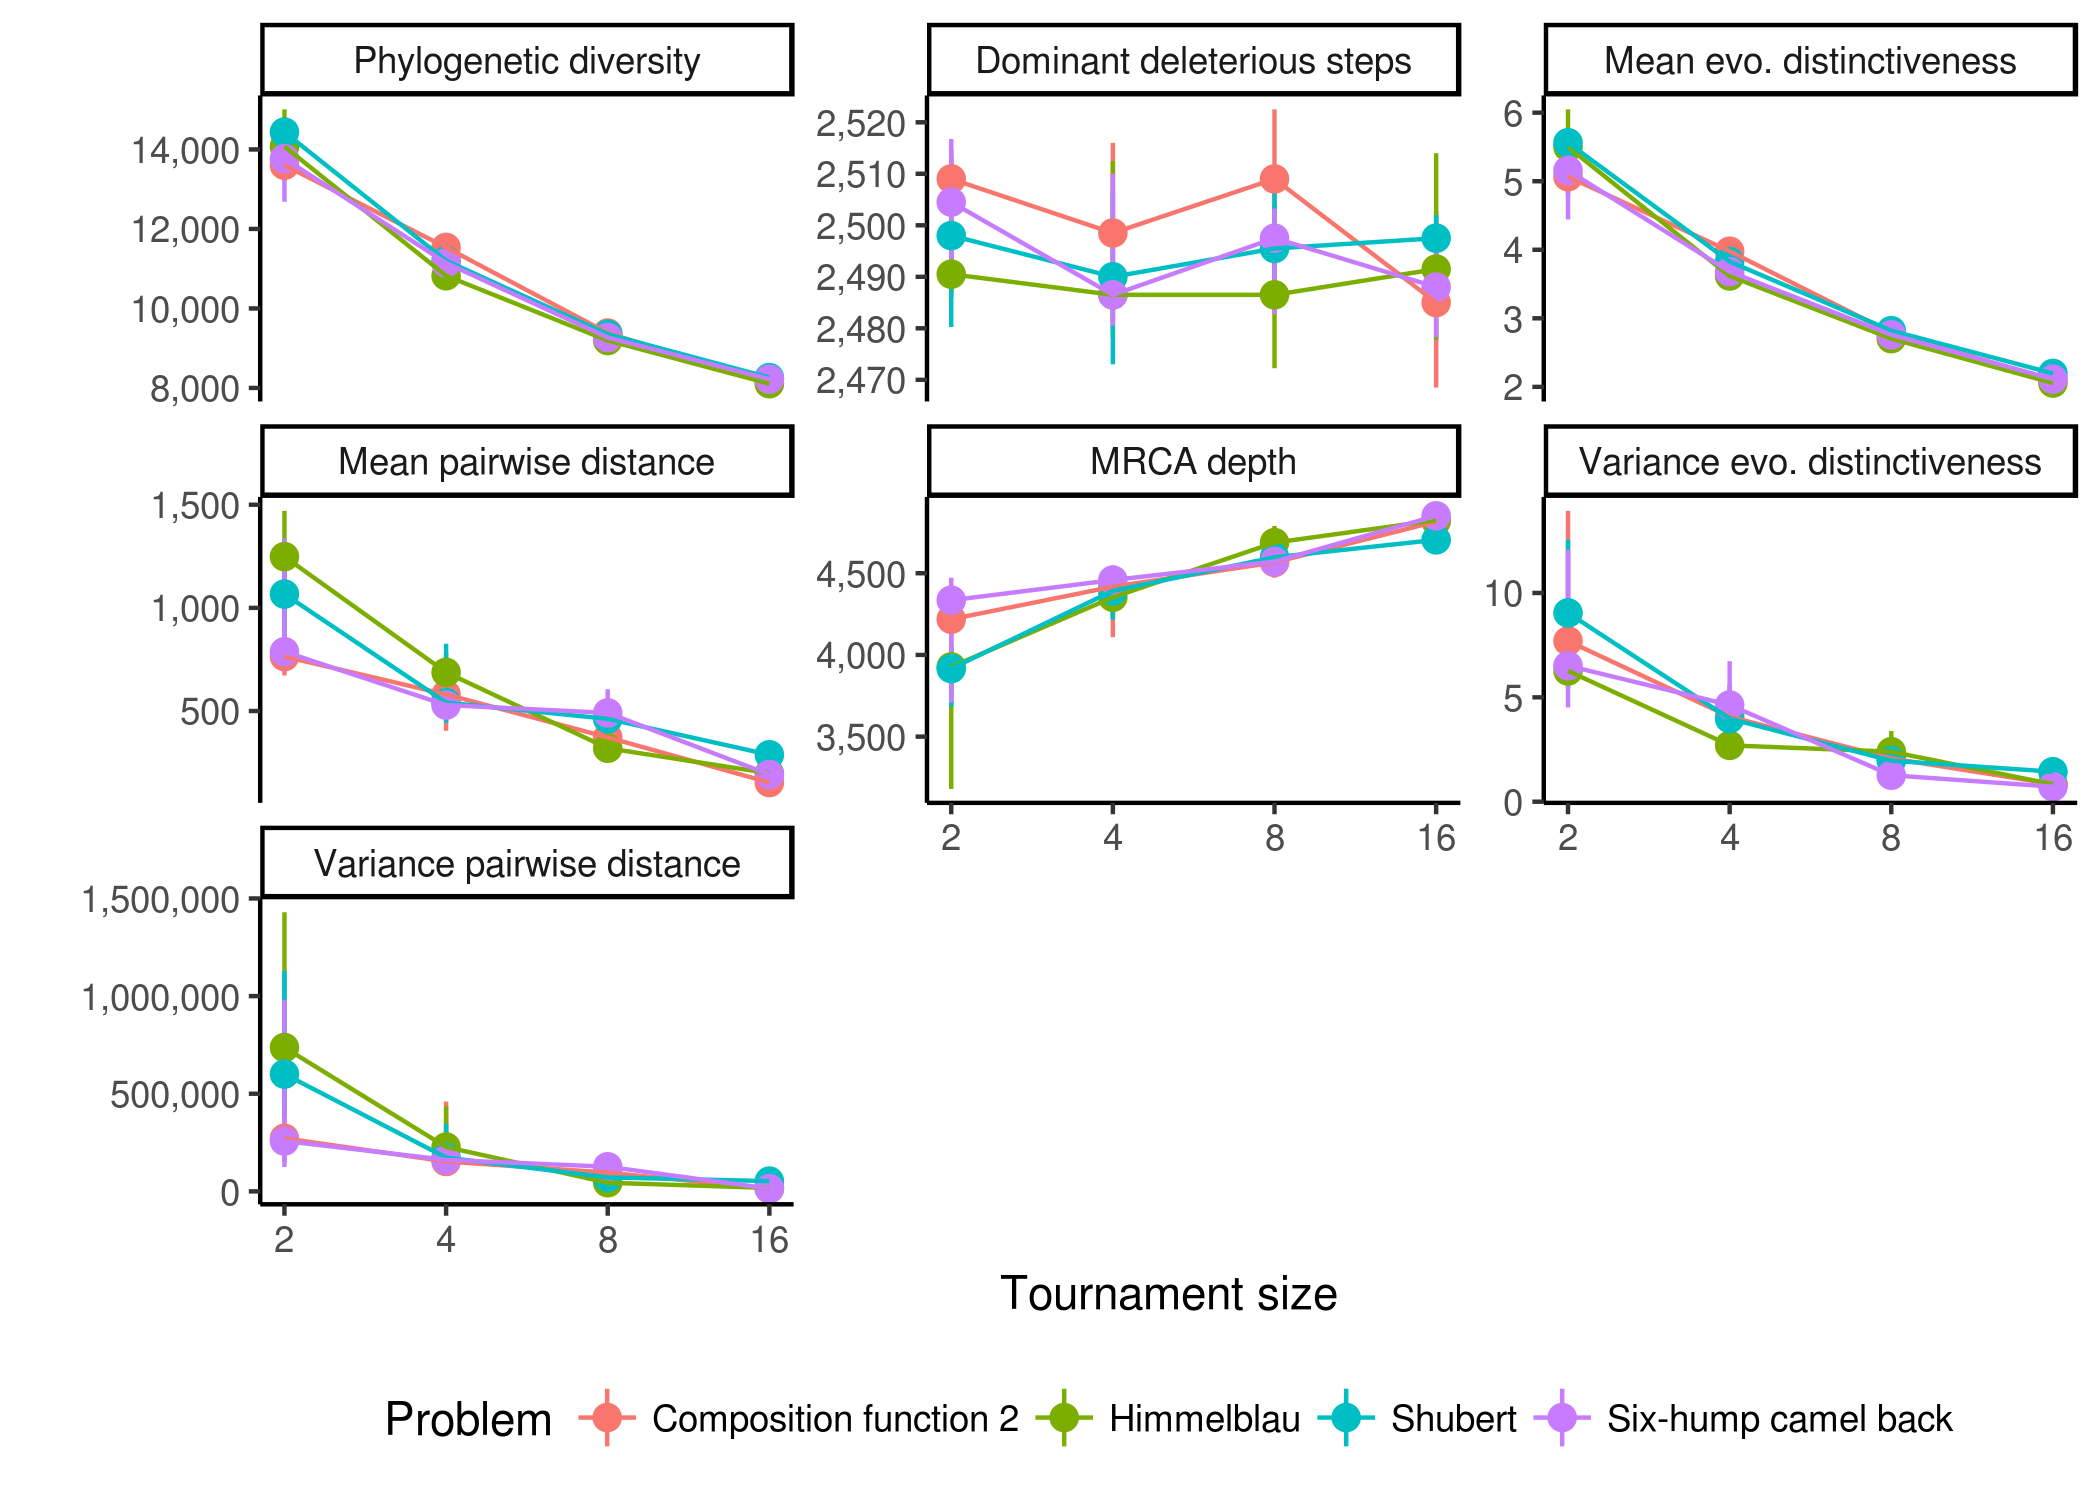
\includegraphics[width=7in]{figs/all_ts.png}
\caption{Values of example metrics across different tournament sizes for each of the four problems. Circles are medians and vertical lines show inter-quartile range.}
\end{figure*}
% \begin{figure}
% 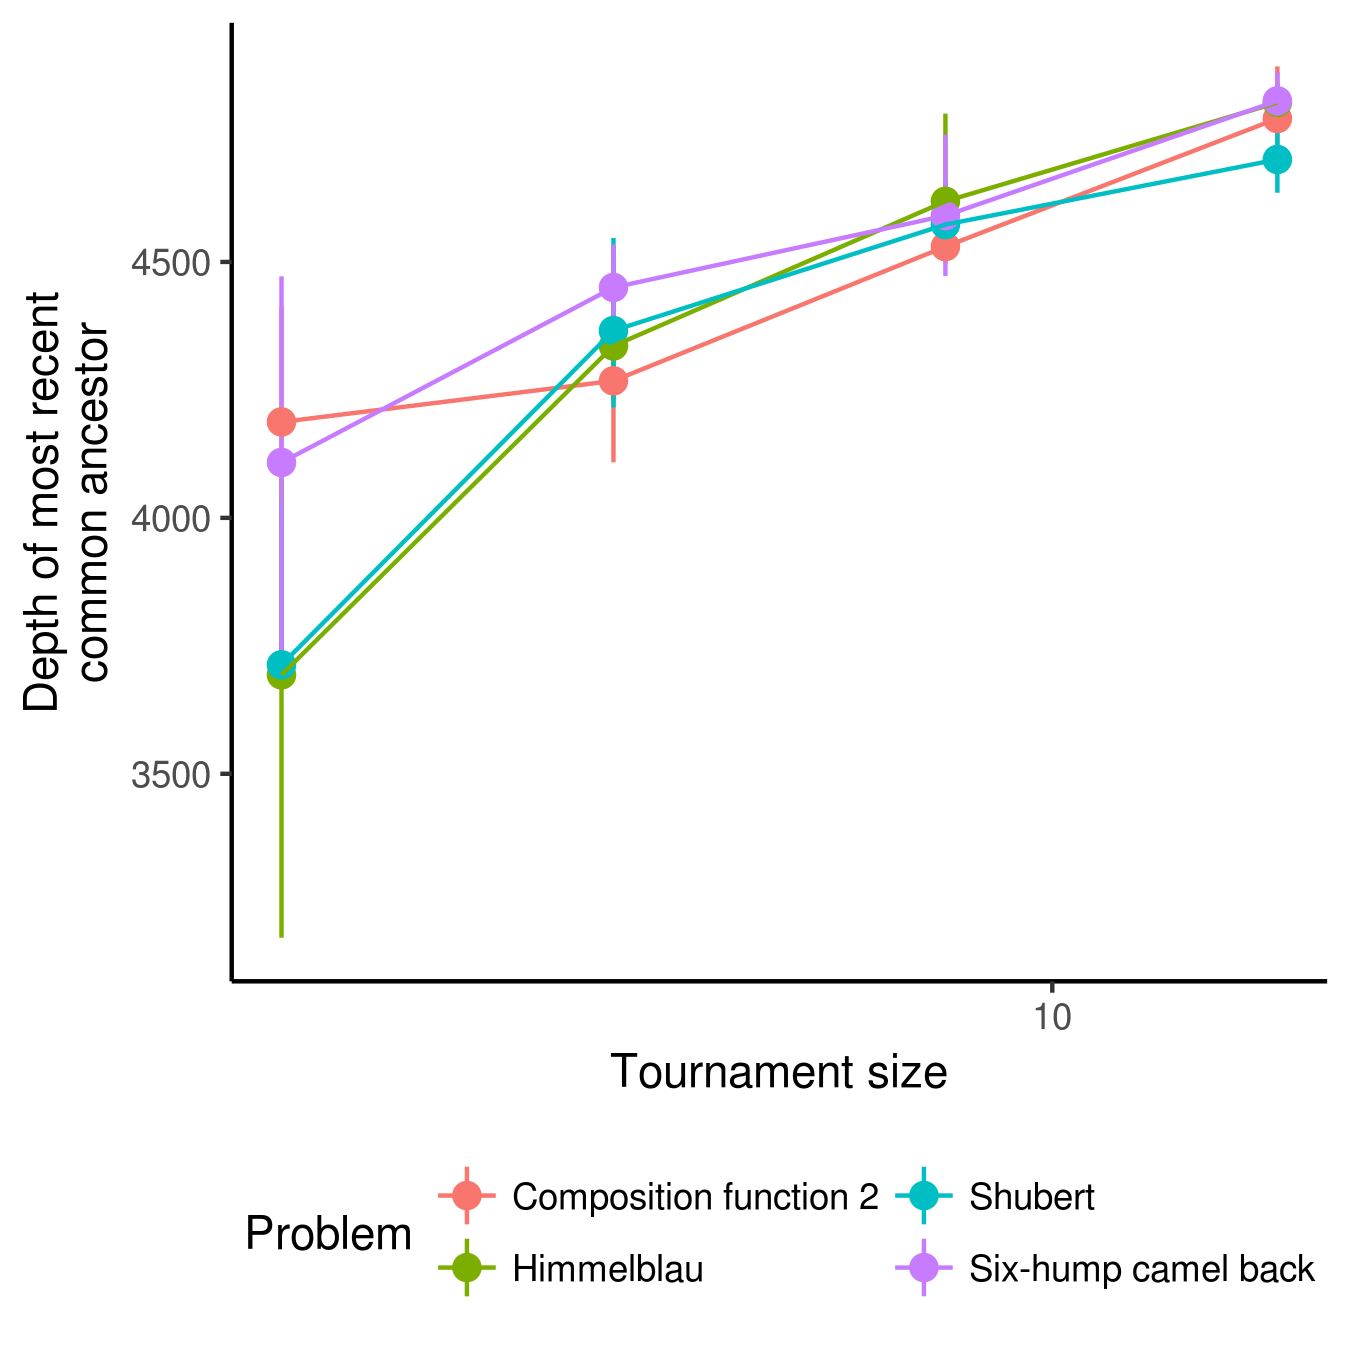
\includegraphics[width=3.5in]{figs/mrca_ts.png}
% \end{figure}

% Changing selection
% - Metric 1
% Problem 1
% Problem 2
% Problem 3
% Problem 4
% - Metric 2

\section{Conclusions}

\section{Acknowledgements}


\footnotesize
\bibliographystyle{apalike}
\bibliography{Zotero,bibliography} % replace by the name of your .bib file

\end{document}
